\documentclass[deutsch]{llncs}
\usepackage{multirow, cellspace}
\usepackage{microtype}
\usepackage{tabularx}
\usepackage{ltablex}
\usepackage{amssymb}
\usepackage{amsmath}
\usepackage[utf8]{inputenc} %Umlaute
\usepackage{amssymb}
\usepackage{upgreek}
\usepackage{graphicx}
\usepackage{amsmath}
\usepackage{array}
\usepackage{gensymb}
\usepackage{enumerate}

% subfigure
\usepackage{caption}
\usepackage{subcaption}
%

\usepackage{adjustbox}
\usepackage{diagbox}
\usepackage{pgfplots}

\renewcommand{\arraystretch}{1.5}
\setlength{\jot}{10pt}

\begin{document}

\title{Intelligente Sehsysteme - Übungsblatt 8}


\author{Hendrik Walther, Jan Konrad}
\institute{}
\maketitle
\section{ImageToolBox: Gamma-Korrektur}
\begin{enumerate}
	\setcounter{enumi}{1}
	\item Eine Gamma-Korrektur mit $\gamma=3$ dunkelt das Bild ab. \\
	      Der Verlauf der Korrekturfunktion zeigt, dass niedrige Intensitätswerte gestaucht werden: $[0,0.5] \rightarrow [0,0.2]$\\
	      Hohe Intensitätswerte werden gespreizt: $[0.8,1] \rightarrow [0.5,1]$ \\

	      Eine Gamma-Korrektur mit $\gamma=1$ hat keinen Effekt. \\
	      Der Verlauf der Korrekturfunktion zeigt, dass jeder Intensitätswert unverändert bleibt: $T_\gamma(I)=I$ \\

	      Eine Gamma-Korrektur mit $\gamma=0.3$ hellt das Bild auf. \\
	      Der Verlauf der Korrekturfunktion zeigt, dass niedrige Intensitätswerte gespreizt werden: $[0,0.2] \rightarrow [0,0.6]$\\
	      Hohe Intensitätswerte werden gestaucht: $[0.5,1] \rightarrow [0.8,1]$
\end{enumerate}

\begin{figure}
	\centering
	\begin{subfigure}{.32\textwidth}
		\centering
		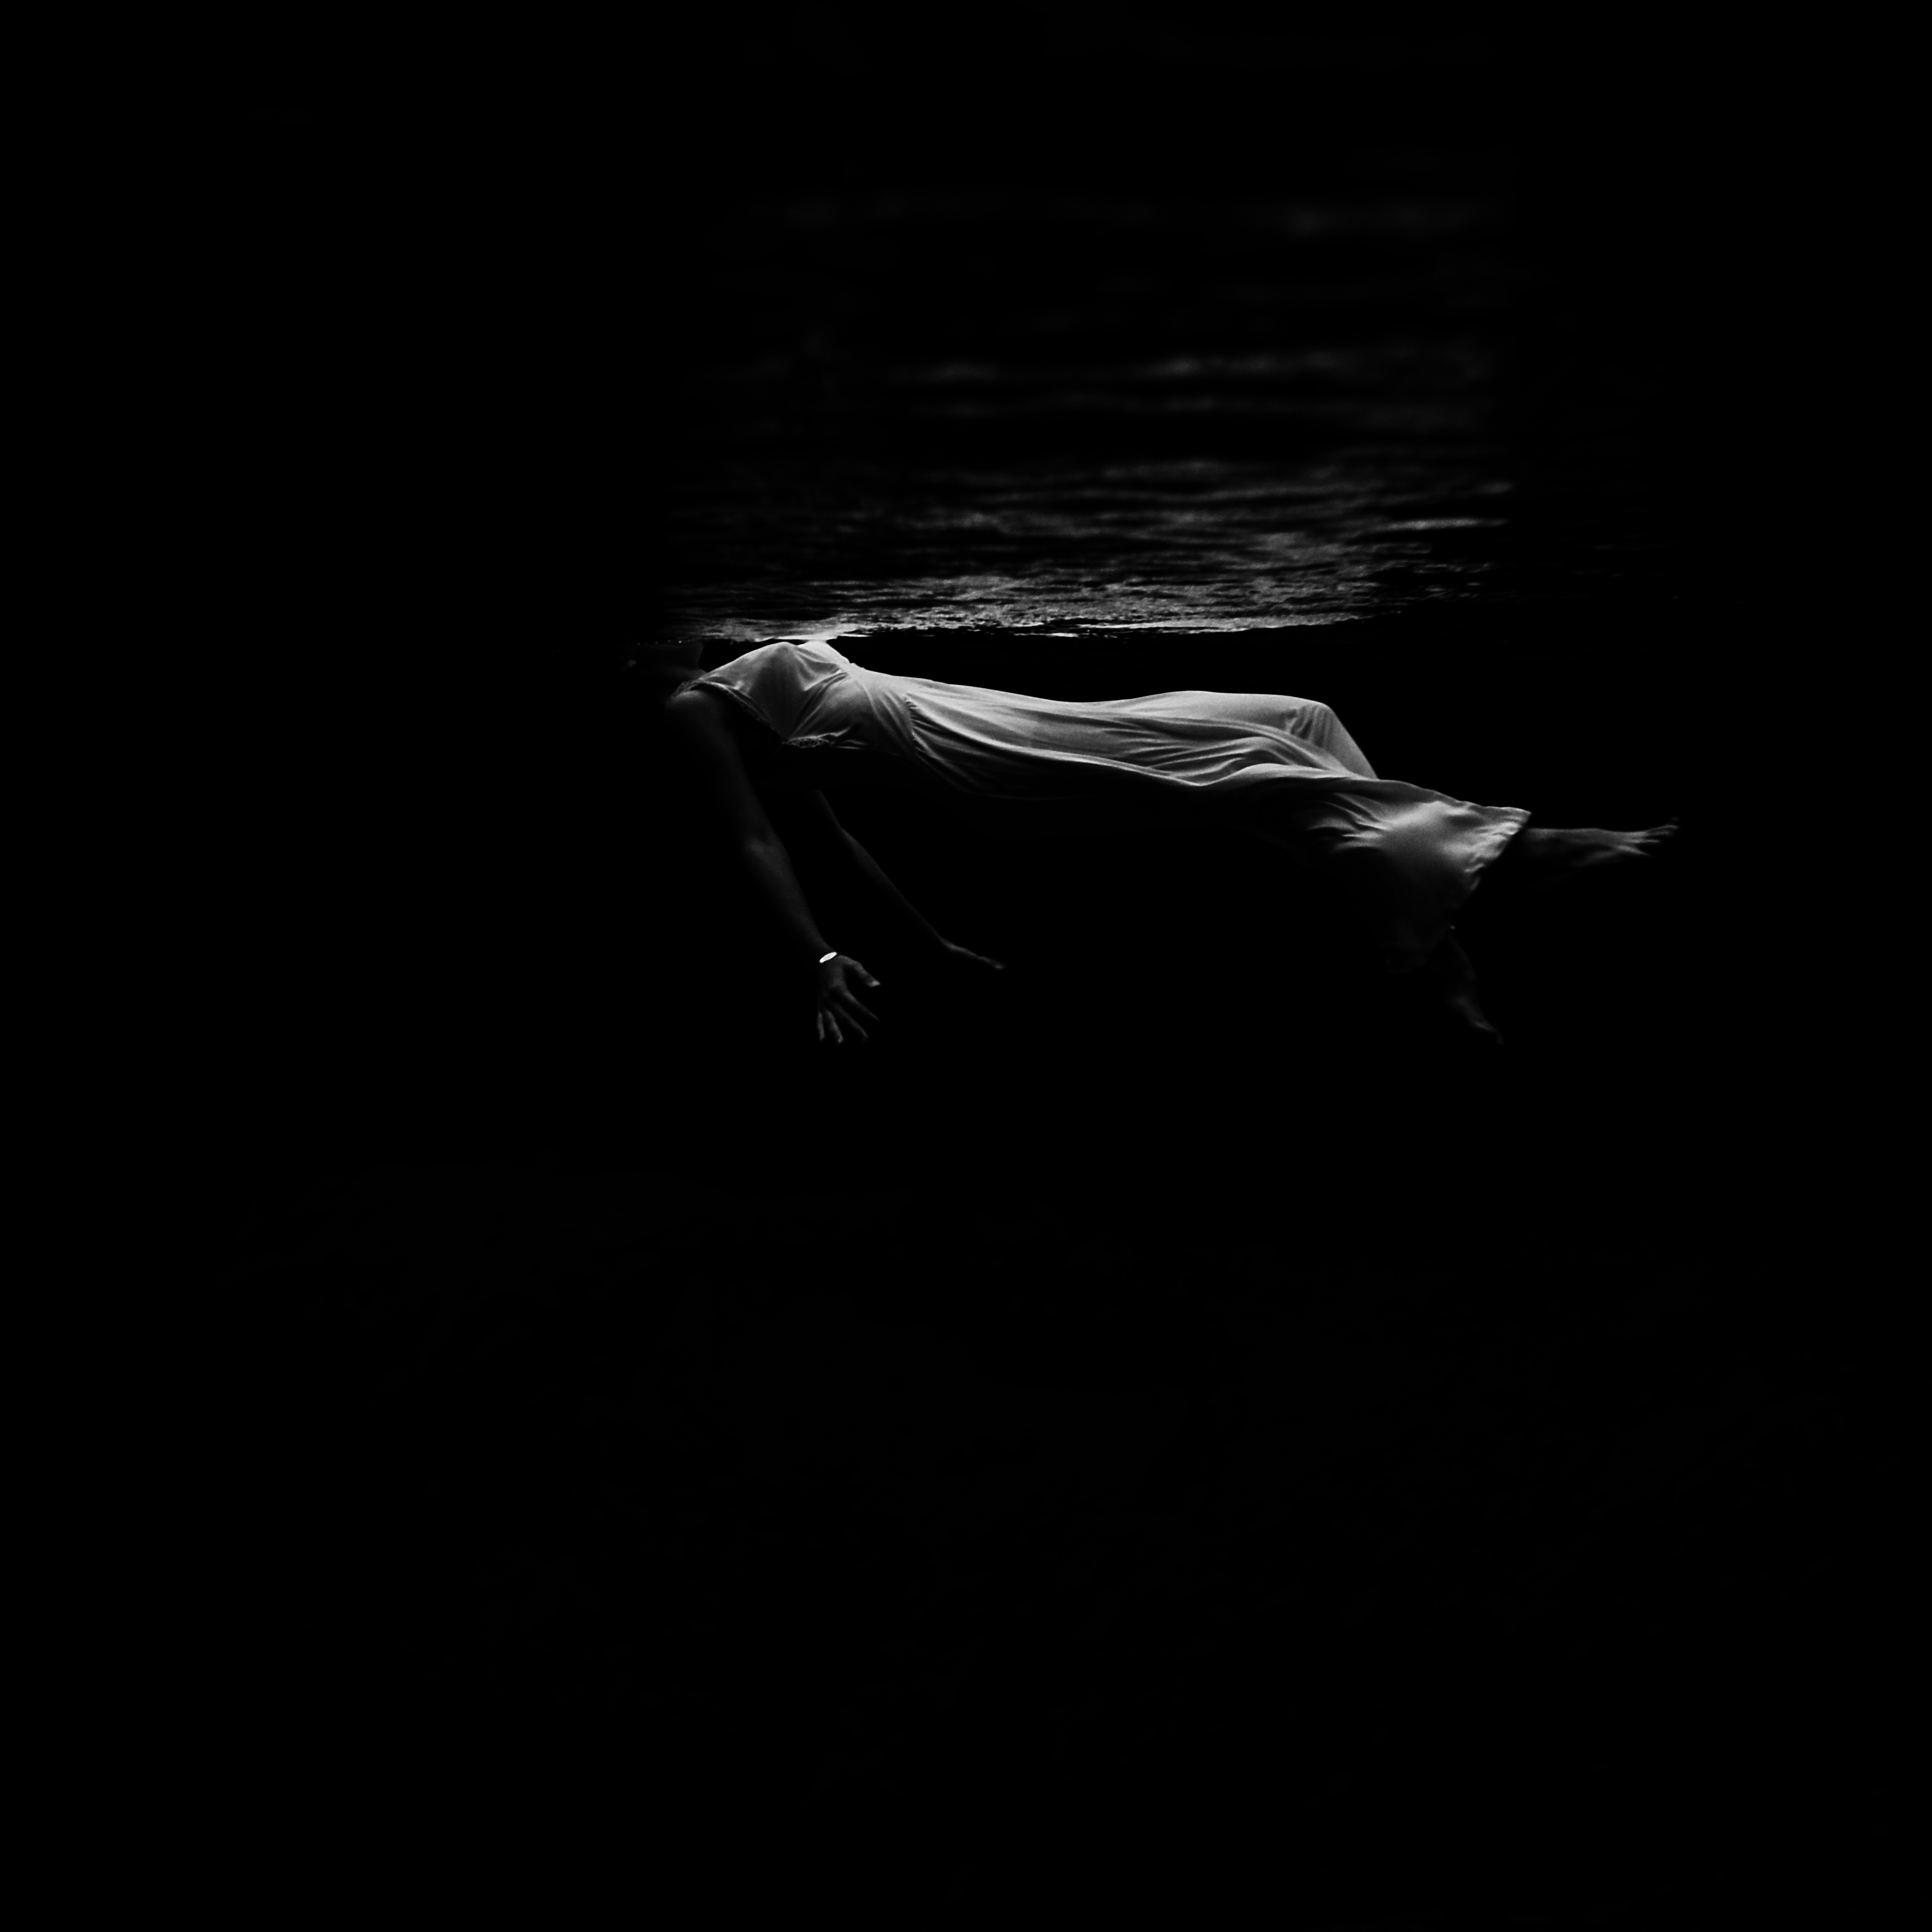
\includegraphics[width=.99\linewidth]{A1/gamma=3.png}
		\caption{$\gamma=3$}
	\end{subfigure}
	\begin{subfigure}{.32\textwidth}
		\centering
		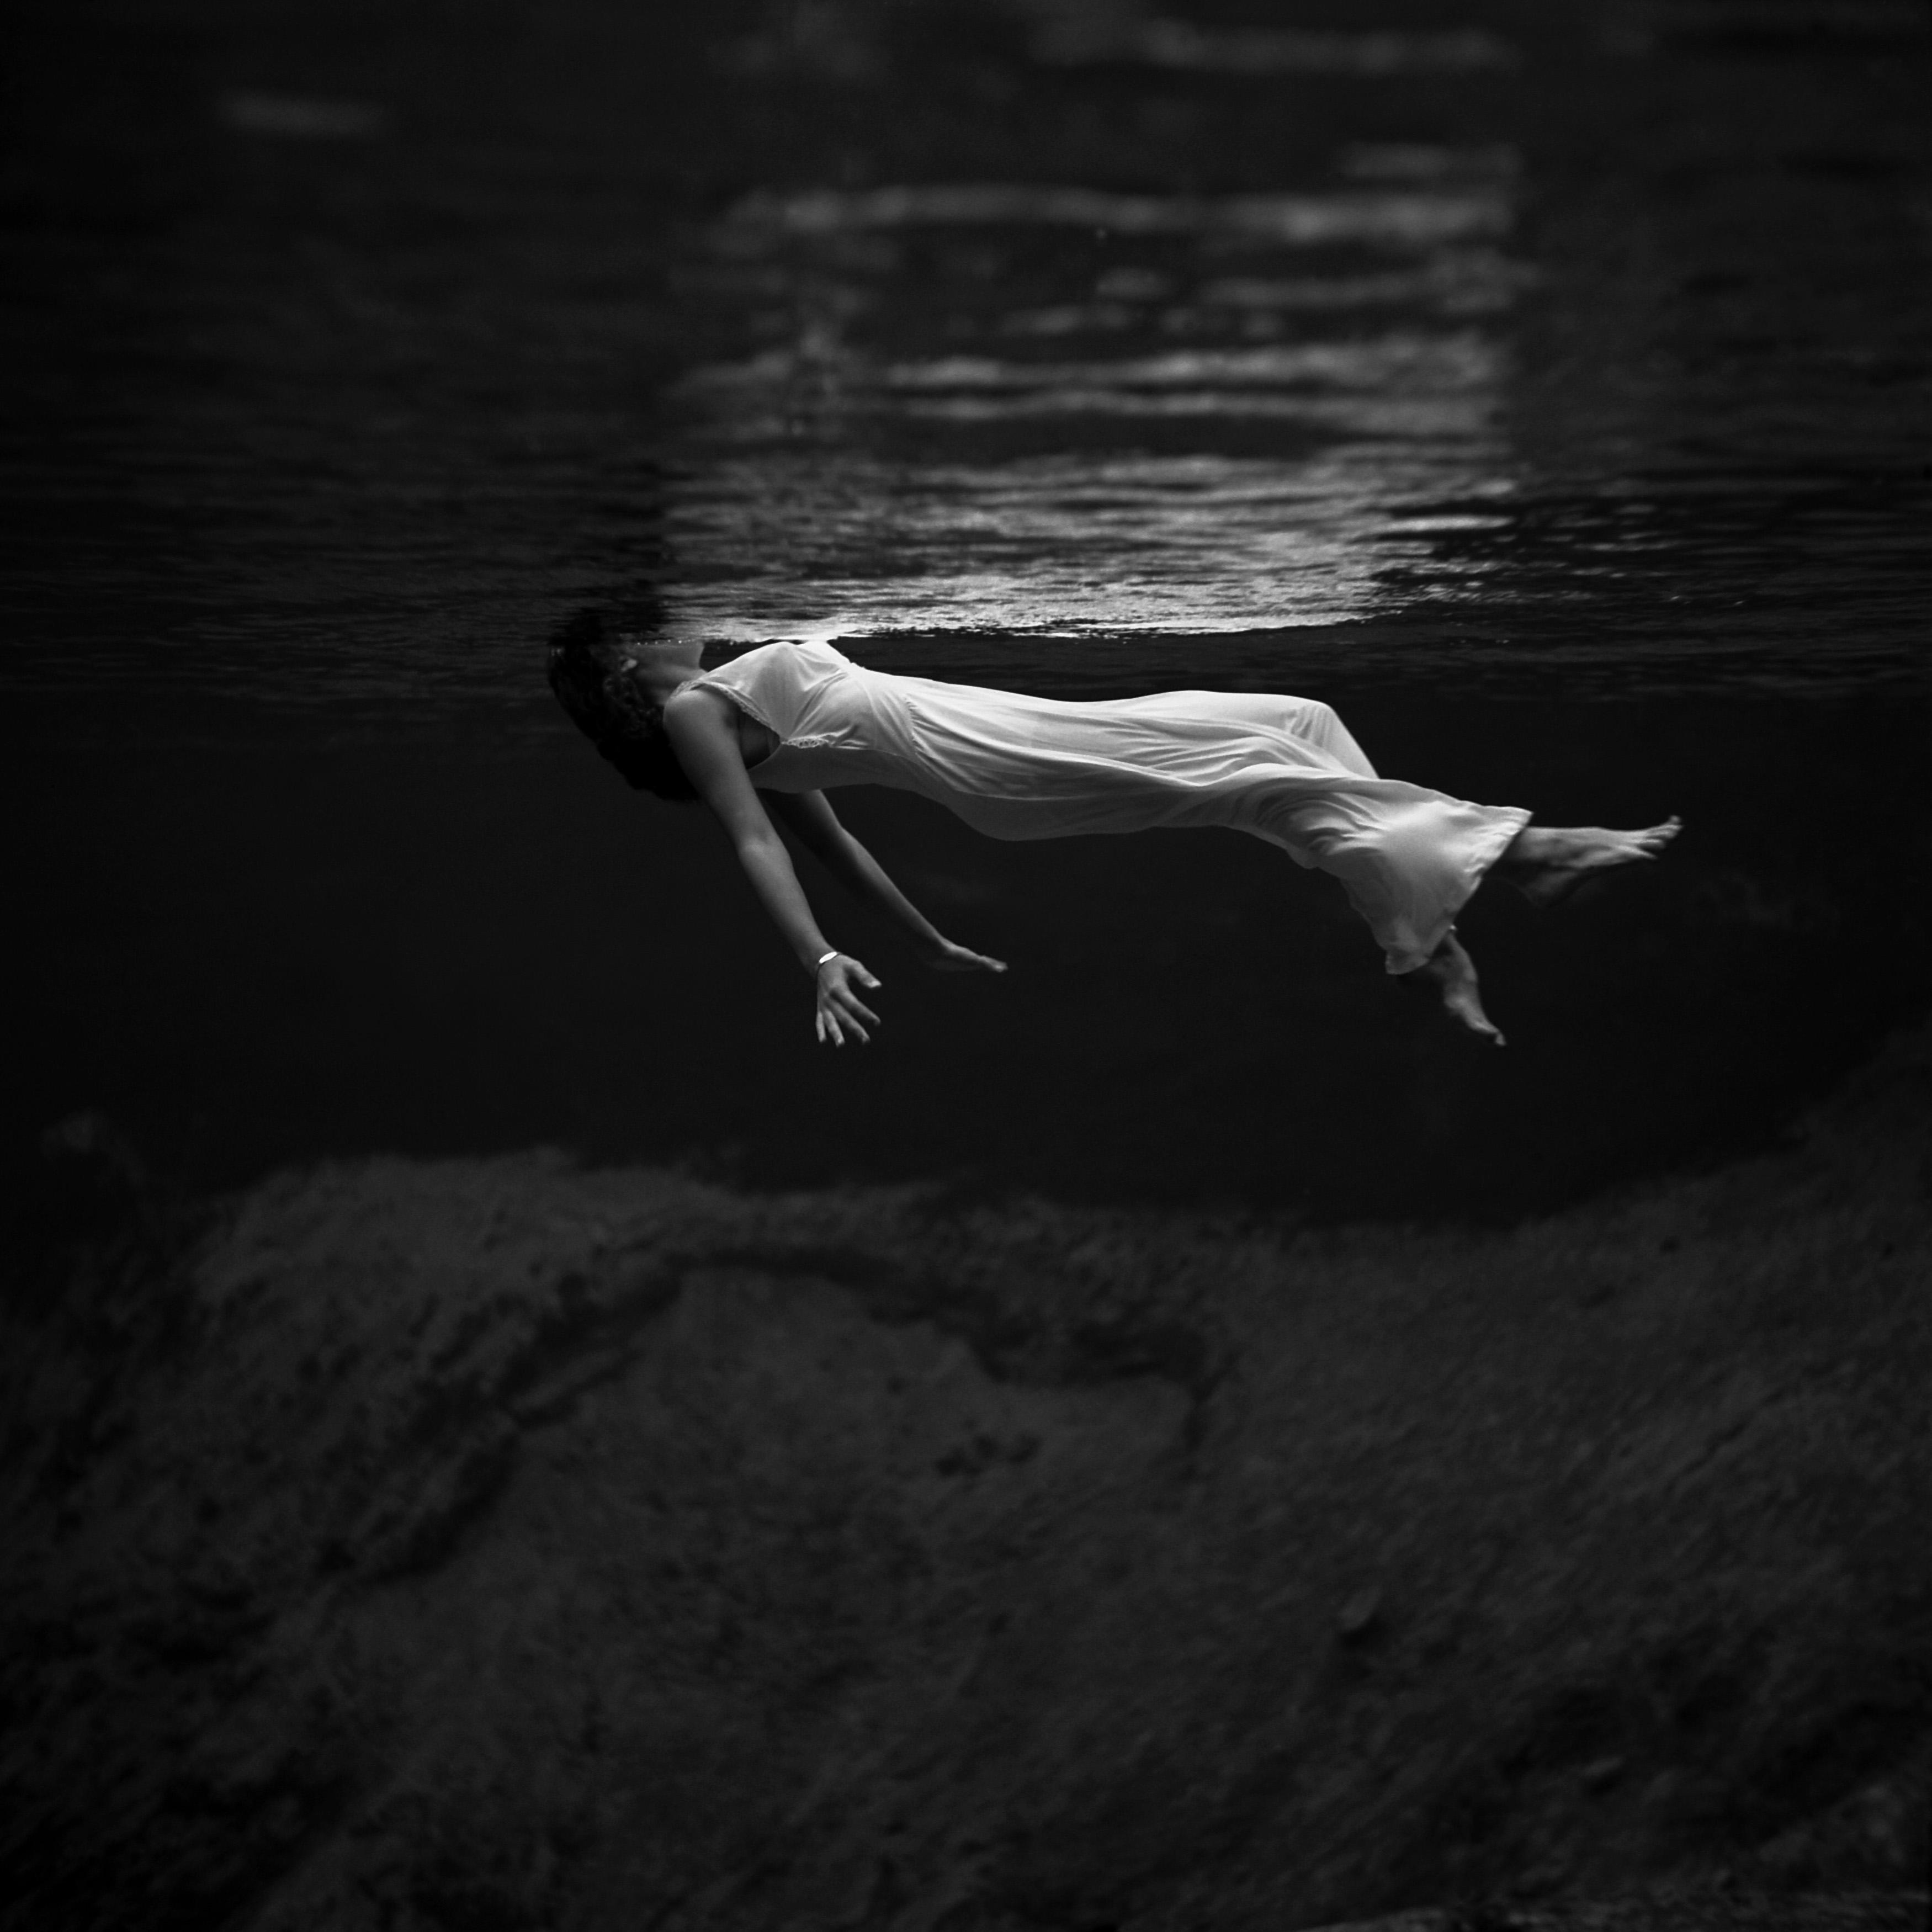
\includegraphics[width=.99\linewidth]{A1/gamma=1.png}
		\caption{$\gamma=1$}
	\end{subfigure}
	\begin{subfigure}{.32\textwidth}
		\centering
		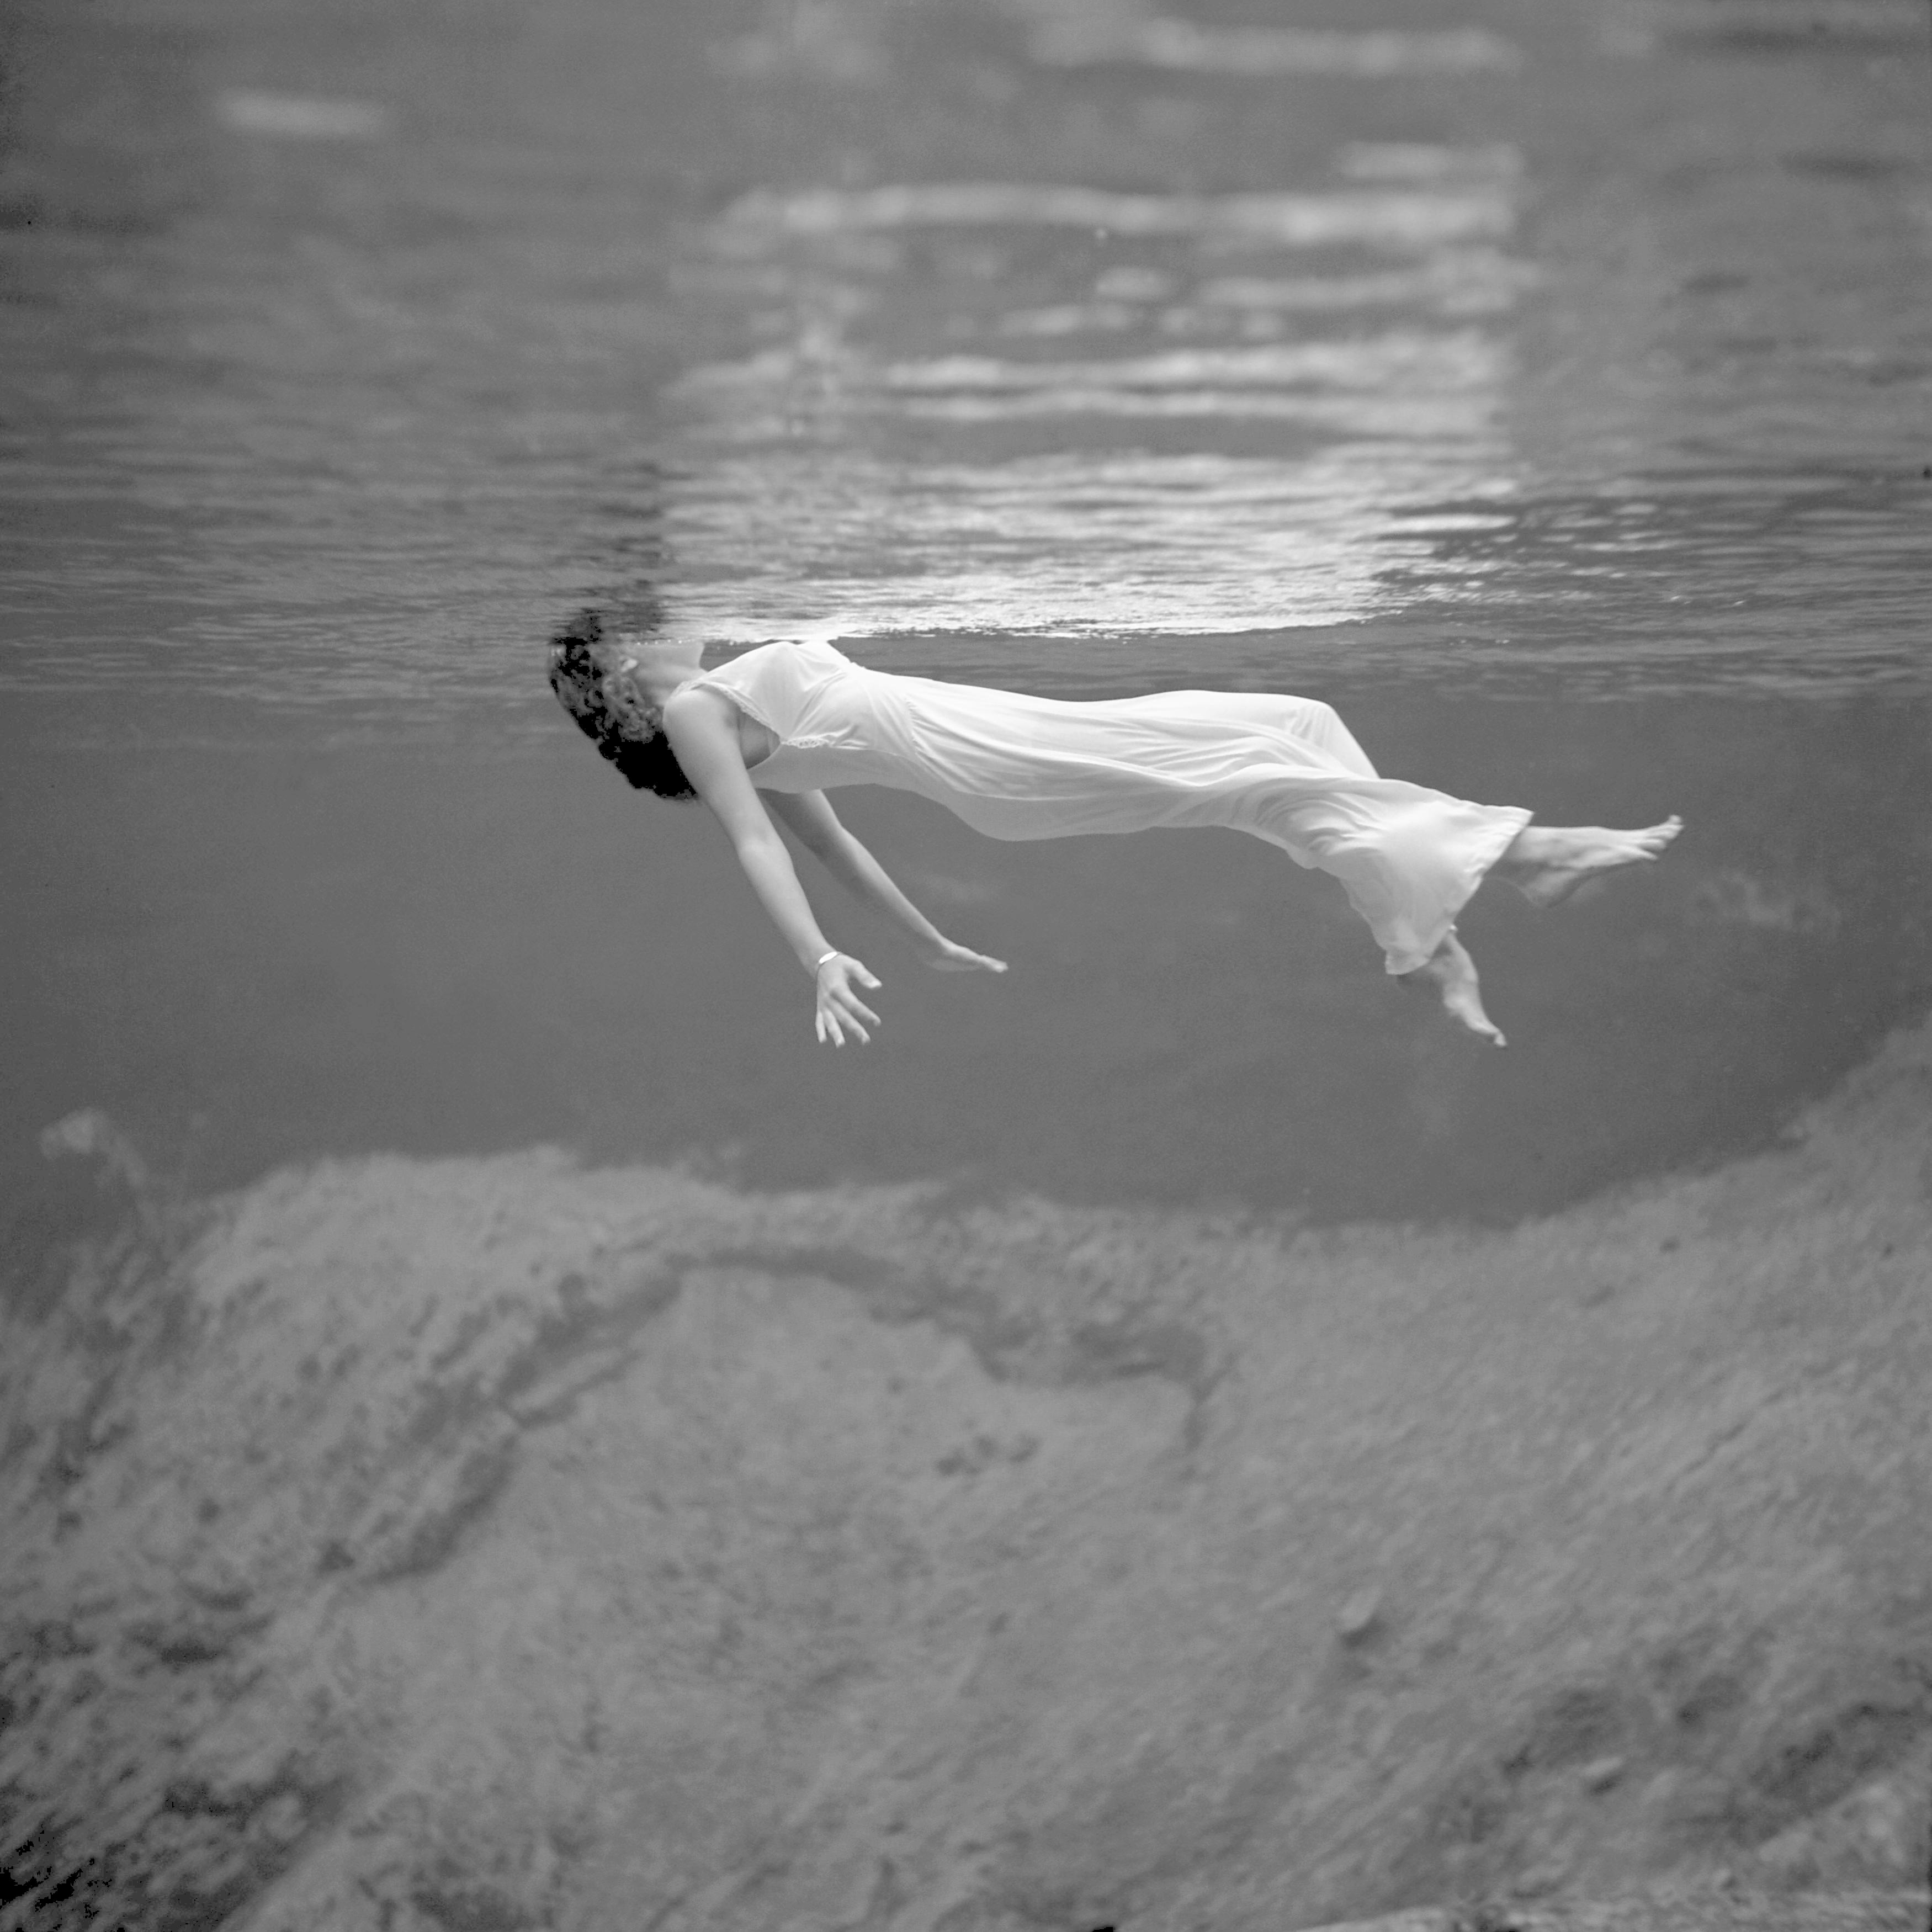
\includegraphics[width=.99\linewidth]{A1/gamma=0.3.png}
		\caption{$\gamma=0.3$}
	\end{subfigure}
\end{figure}
\newpage
\setcounter{section}{2}
\section{ImageToolBox: Diffusionsfilter }

\begin{figure}
	\centering
	\begin{subfigure}{.49\textwidth}
		\centering
		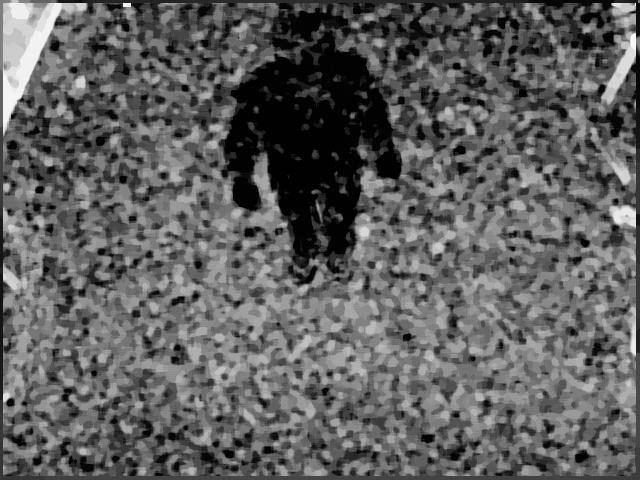
\includegraphics[width=.99\linewidth]{A3/lambda0.5.jpg}
		\caption{$\lambda=0.5$}
	\end{subfigure}
	\begin{subfigure}{.49\textwidth}
		\centering
		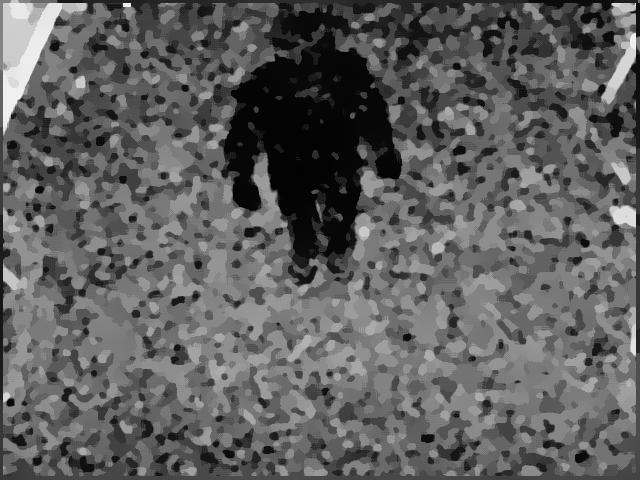
\includegraphics[width=.99\linewidth]{A3/lambda1.jpg}
		\caption{$\lambda=1$}
	\end{subfigure}
	\begin{subfigure}{.49\textwidth}
		\centering
		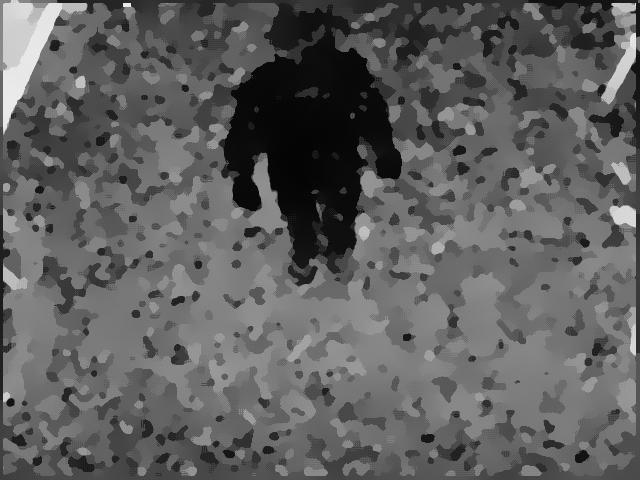
\includegraphics[width=.99\linewidth]{A3/lambda1.5.jpg}
		\caption{$\lambda=1.5$}
	\end{subfigure}
	\begin{subfigure}{.49\textwidth}
		\centering
		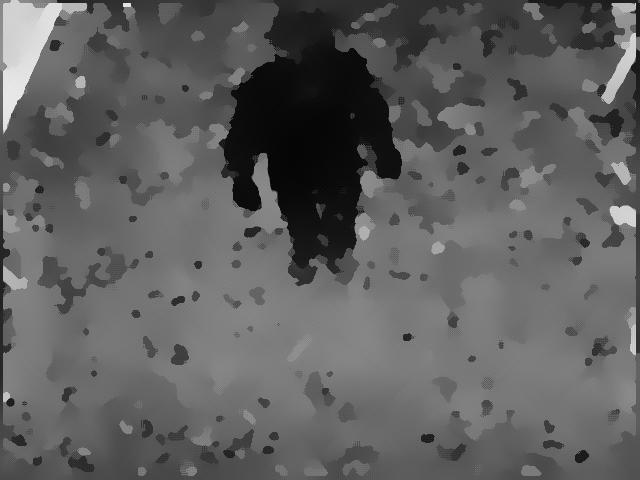
\includegraphics[width=.99\linewidth]{A3/lambda2.jpg}
		\caption{$\lambda=2$}
	\end{subfigure}

	\caption{Isotropes inhomogenes Diffusionsfilter mit $\epsilon_0=1$ und 500 Iterationen}
\end{figure}

\end{document}
